\chapter{Introduction} \label{chapter:intro} 
Recent years have witnessed a tremendous growth in the use of accelerators in computer systems to improve the systems' performance and energy efficiency \cite{kim2014compression, majumder2014hardware, iouliia2004reconfigurable, souradip2010hardware, putnam2014reconfigurable}. Among these accelerators, GPUs and Xeon Phi accelerators have stood out as two of the most popular choices in spite of their relatively short history as accelerators--5 of the top 10 systems on the top500 list take advantage of them \cite{top500}. On the other hand, despite the long and successful track record of FPGA accelerators with promising performance speedup and energy efficiency \cite{iouliia2004reconfigurable, souradip2010hardware, asano2009performance, che2008accelerating, thomas2009comparison}, the use of FPGA accelerators in main-stream systems remains limited and has yet to receive widespread adoption beyond highly skilled hardware engineers \cite{cong2011high}. When compared to the wide adoption of GPUs and Xeon Phi accelerators, it is believed that the much lower design productivity in developing FPGA applications, which is generally caused by both the lengthy FPGA compilation and notorious inaccessibility to software programmers, has become one of the major obstacles that hinder the software developers using FPGAs as compute accelerators. 

When considering the classical hardware description language (HDL) based FPGA accelerator development flow, a number of aspects lead to the FPGA design productivity challenge. First of all, the FPGA design process using HDL is fundamentally different from that of software development and requires the low-level circuit design techniques which most of the software designers are unfamiliar with. In addition, the relatively low abstraction level of hardware description languages also limits the efficiency of the application development and thus the designers' productivity eventually \cite{cong2011high}. Secondly, instead of spending seconds to compile and debug a quick-and-dirty proof-of-concept design, software programmers soon find that implementing even the smallest FPGA design consumes at least tens of minutes. As the size of their designs increases, the run-time of the implementation tools quickly goes up to hours or even days, greatly limiting the number of possible debug-edit-compile cycles per day \cite{lavin2010using, lavin2011HMFlow, korf2011automatic, yue2015rapid}. Beyond that, software designers are often put off by the large amount of design optimization options involved in both the design tools and the hardware designs. Moreover, the initial hardware design can rarely meet the requirements and the design optimization is critical to achieve the anticipated performance and energy-efficiency \cite{schafer2012machine, zhong2014design, holzer2007design, schafer2012divide, liu2013learning, kurek2014automating}. 

Although both the industry and academia have made significant progress in increasing the productivity of the FPGA designers by improving the EDA tools for shorter run time \cite{VivadoHLS, mulpuri2001runtime, moctar2014parallel, goeders2011deterministic} and providing a large amount of IPs for design reuse \cite{xilinx-pc, altera-pc}, the typical FPGA compilation remains two orders of magnitudes slower than software compilation and the FPGA accelerator design remains a discipline mostly carried out by highly trained specialists. The full potential of FPGAs to the software programmers hasn't been fully unleashed and there is still a long way to drive towards software programmable FPGA allowing high-productivity FPGA development \cite{fsp2014, fsp2015}.

\section{High-level Synthesis}
To bridge the design productivity gap between software and hardware development, many people have turned to the use of high-level synthesis (HLS) techniques in the past decades \cite{cong2011high}. \figref{fig:hls-compilation} presents both the FPGA design flow using conventional hardware description language (HDL) and HLS. It is clearly that the HDL based FPGA design flow takes HDL as the design entry and thus requires the users to be experienced on low-level circuit design to develop a register-transfer level (RTL) FPGA accelerator for an application. By raising the abstraction level of the physical hardware, HLS based design flow allows designers to develop hardware using familiar high-level, software-like description languages such as C, C++, C-like languages, Matlab and Python \cite{handel-c, ROCCC, VivadoHLS, OpenCL, matlab, myhdl}. The low-level hardware implementations are then left to the conventional design tools to synthesize and optimize. With decades of efforts, some early results in HLS have already found their ways into FPGA vendors' commercial tools in recent years \cite{OpenCL, VivadoHLS, handel-c, zhang2008autopilot, chen2005xpilot}. 

\begin{figure}
\centering
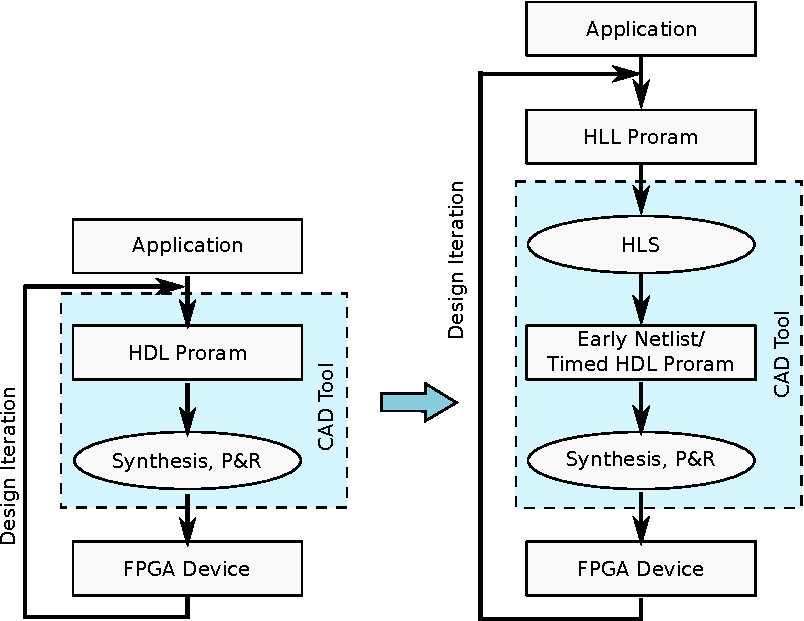
\includegraphics[width=0.65\linewidth]{hls-compilation}
\caption{FPGA Design Flow Using Conventional HDL and HLS.}
\label{fig:hls-compilation}
\end{figure}

Unfortunately, when considering the overall design productivity of developing hybrid hardware/software applications, the raised abstraction provided by HLS is only addressing part of the problem. While the high-level abstraction makes expressing complex functionality on FPGA easier, the lengthy compilation spent in synthesis, placing and routing remains a bottleneck to the overall design productivity for designers who are accustomed to the high speed software compilation. As shown in \figref{fig:hls-compilation}, whenever the target application changes to a similar one or even the single application changes slightly during its design iterations, the lengthy compilation process must be repeated. Therefore, the lengthy compilation is dramatically impacting the possible debug-edit-compile cycles achievable per day and thus the design productivity of a designer.  

\section{Overlay Architecture}
Recently there has been an increased interest in employing the concept of overlay architectures which are essentially virtual architectures (VA) overlaying on top of physical architectures (PA) i.e. FPGAs as a way to approach this design productivity challenge \cite{olaf2013, coole2010intermediate, lin2012energy, jain2015efficient, liu2015automatic, brant2012ZUMA, lebedev2010MARC, kissler2006dynamically, ferreira2011fpga, jeffrey2011potential, capalijia2013pipelined, koch2013efficient, coole2015adjustable, grant2011malibu}. VA overlay locates between the user application and the underlying physical FPGA similar to that shown in \figref{fig:overlay-concept}. With this intermediate VA layer, user applications will be targeted toward the overlay architecture regardless of what the physical FPGA may be. A separate step will subsequently translate this VA overlay, together with the application that runs on VA, on to the PA layer. On the other hand, the overlay built on top of PA layer can be reused for design iterations of the application development or different applications that are mapped to the same PA layer, which helps to amortize the overlay building time and improve the design productivity eventually.

\begin{figure}
\centering
\includegraphics[width=0.5\linewidth]{overlay-concept}
\caption{Overlay Based 2-layer Approach to FPGA Application Development. Overlay may be designed as a virtual FPGA, or it may implement an entirely different compute architecture such as a coarse-grained reconfigurable array (CGRA), vector processor, multi-core processor, or even a GPU.}
\label{fig:overlay-concept}
\end{figure}

Taking advantage of FPGA's general-purpose configurability, many researchers have demonstrated the benefits of diverse overlays such as virtual FPGAs \cite{brant2012ZUMA, grant2011malibu, coole2010intermediate}, soft processors \cite{nios, microblaze, guy2012VENICE}, massive parallel processing arrays (MPPAs) \cite{kissler2006dynamically, boppu2014compact, hannig2014invasive}, many-core processor system \cite{lebedev2010MARC}, coarse-grained reconfigurable arrays (CGRAs)\cite{lin2012energy, jain2015efficient, capalijia2013pipelined} and even graphic processing units (GPUs) \cite{al-dujaili2012Guppy}. With the overlays especially the ones that have coarser granularity, software programmers are now possible to utilize the FPGAs as accelerators simply by writing programs that target a familiar computing architecture instead of working with unfamiliar hardware-centric FPGA programming paradigms. In general, one significant benefit of using FPGA overlay is to bridge the gap between the software programmers and the low-level FPGA hardware fabric. In addition, the overlay architecture helps to hide the physical FPGA details from the application. Therefore the user designs targeting the overlay are portable to FPGAs of different parts and from different vendors.

Of course, if an application is ready to be accelerated on a advanced computing architecture overlay implemented using FPGAs, then it is understandable to come up the question: why not simply run the application on such a high-performance hard computing architecture instead. The answer to this question is actually the key of the overlay research. Not only does the overlay offer desirable software-programmable fabrics on top of physical FPGAs, it also takes advantage of the inherent programmability of the physical FPGA allowing the overlay to be specifically customized to an application or a group of applications concerned for the sake of both performance and energy efficiency. Although the overlay inevitably introduces additional performance penalty and hardware resource cost, a good overlay must ensure that the performance of the resulting overlay based design remains competitive for the accelerator system to be worthwhile while the increasingly larger FPGAs with millions of programmable elements \cite{virtex-ultrascale} are also able to afford the overlay resource overhead.

\section{Soft CGRA Overlay Based FPGA Accelerator}
This dissertation work aims to provide a rapid FPGA accelerator design framework by using an overlay pre-built on top of physical FPGAs while maintaining competitive performance of the resulting system at the same time. Since general purpose processor remains a better choice for complex applications such as OS and GUI environment while FPGA is preferable for compute-intensive loop kernels which are usually performance bottleneck in many applications such as signal processing, image processing, scientific computing and financial computing \cite{sukhsawas2004high, bouris2010fast, wu2009fine, tian2008high}. Thereby, this work targets a hybrid CPU-FPGA computing system and followed the common wisdom offloading the compute intensive loop kernels to the FPGA accelerator while leaving the rest part of the applications on a general purpose processor \cite{baleani2002HW-SW, canis2011legup}. In particular, instead of adopting general FPGAs for random application acceleration, a soft CGRA (SCGRA) overlay is developed for rapid FPGA accelerator design targeting only simple nested loop kernels as demonstrated by numerous CGRA design on application specific integrated circuit (ASIC) \cite{compton2002reconfigurable, tessier2001reconfigurable}.  

The proposed FPGA loop accelerator design framework is named QuickDough as shown in \figref{fig:qd-overview}. It takes high-level user-designated loop kernels as input and then maps the loop kernels to the SCGRA overlay based FPGA accelerators. As the SCGRA overlay has coarser configuration granularity than the physical FPGAs, mapping high-level loop kernels to the SCGRA overlay is much faster compared to the direct mapping from the equivalent HDL program to the FPGA directly. In addition, to reduce the lengthy accelerator implementation (i.e. synthesis, placing and routing) time, a representative SCGRA overlay based FPGA accelerator library is pre-built. As the library can be reused by a domain of applications or design iterations of an application, the lengthy FPGA accelerator implementation can be amortized allowing rapid FPGA loop accelerator generation. Meanwhile, QuickDough also produces communication interface between the host processor and the resulting accelerator, which can be easily called by the original high-level applications. Consequently, the original high-level application can be compiled to the target hybrid CPU-FPGA computing system.

\begin{figure}
\centering
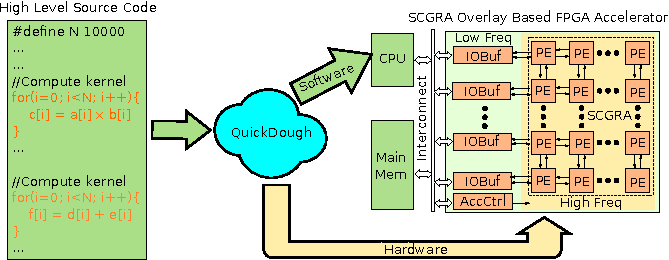
\includegraphics[width=0.9\linewidth]{qd-overview}
\caption{QuickDough Overview, it takes user-designated loop kernels as input and generates corresponding hardware acceleration system through a soft CGRA overlay targeting a hybrid CPU-FPGA computing system.}
\label{fig:qd-overview}
\end{figure}

The SCGRA overlay is the backbone of the generated accelerators and has great influence on both performance and energy efficiency of the resulting acceleration system developed using QuickDough. In this work, a template of SCGRA consisting of an array of processing elements (PEs) is developed. It takes advantage of the inherent configurability of the FPGAs and provides just enough functionality to meet the requirements of the target application or a domain of applications. It is clear that the SCGRA is light-weight, soft and different from the conventional CGRAs with composable functionality which have to support all the features on the silicon. The SCGRA template is highly pipelined to provide high implementation frequency and good performance of the resulting accelerators accordingly. At the same time, it is simple, flexible and scalable to ensure convenient customization for less resource consumption and higher energy efficiency. 

One of the key advantages of using the SCGRA overlay for loop acceleration is the capability to customize the overlay specifically to an application or a domain of applications for higher performance and better energy efficiency. Otherwise, compiling the loop kernels to the SCGRA overlay based FPGA accelerators will not be as useful. However, the compilation process involves a labyrinth of architectural and compilation options and exploring such a complex and large design space is a slow and non-trivial process. To require a user to manually explore the design space is going to counteract the design productivity benefit of using overlay in the first place. To address this problem, QuickDough also supports intensive customization of the design parameters including both the compilation options and the SCGRA overlay architectural parameters all the way from high-level loops to corresponding FPGA accelerator bitstream. The customization process is relatively slow yet provides accelerators with optimized performance and energy efficiency. While it is not a frequent process, it may probably be performed at the final application optimization stage.

\section{Project Contribution}
The contribution of the dissertation work mainly includes the following aspects.

\begin{itemize}
\item By utilizing the SCGRA overlay as an intermediate fabric on top of physical FPGA, an FPGA loop accelerator design framework QuickDough that can rapidly produce loop accelerator is proposed. With pre-built accelerator library, a high-level loop kernel can be compiled to the corresponding FPGA accelerator bitstream in seconds dramatically increasing the number of debug-edit-compile cycle per day. When compared to a hard ARM processor, the performance of the resulting accelerators developed using QuickDough achieves up to 10X speedup.

\item A highly pipelined, flexible and scalable SCGRA overlay template is developed. With this template, the generated loop accelerators with various configurations can work at high frequency and achieve higher performance accordingly. The scalability and flexibility of the overlay template makes it convenient to be adapted to a different application which also helps to automate the accelerator generation. 

\item By taking advantage of the regularity of the SCGRA overlay based loop accelerator, the design parameters of the overlay based accelerators from high-level loop unrolling, on-chip buffer sizing and overlay configuration are automatically customized efficiently achieving optimized performance and energy efficiency of the resulting accelerators. Compared with an exhaustive search, the proposed customization method can be two orders of magnitude faster while achieving similar performance.

\end{itemize}

\section{Thesis Roadmap}
In \chapref{chapter:litrev}, the various approaches especially the overlay architectures that were proposed to address the FPGA design productivity challenges in the past decades are summarized. \chapref{chapter:overlay} mainly illustrates the SCGRA overlay template showing the flexible reconfigurability for various applications. Low-level hardware design and optimization especially the pipelining are detailed. In \chapref{chapter:framework}, the proposed FPGA loop accelerator design framework i.e. QuickDough is detailed. Particularly, it focuses on the processes rapidly compiling the high-level nested loops to the corresponding SCGRA overlay based FPGA accelerators. \chapref{chapter:customization} presents a two-step customization method, which efficiently explores the design parameters of the resulting FPGA loop acceleration system on a hybrid CPU-FPGA computing machine by taking advantage of the regularity of the SCGRA overlay based FPGA accelerators. Finally, \chapref{chapter:conclusion} concludes the dissertation and provides insights into future research inspired by QuickDough.
